\section{定位模型：失联后的位置演化}

\subsection{总体框架}

定位模型分两步：\textbf{先按失效模式确定垂向命运}（上浮到水面 / 定深漂流 / 下沉到海底），
\textbf{再做三维输运}（四维流场 + 系统偏差 + 随机扰动 + 海底滑移）。
对每种失效模式各采样若干粒子，合成 30\,000 条轨迹（60 个独立搜救案例 $\times$ 500 粒子）。
每条轨迹的垂向命运由垂向动力学方程决定，水平位置由流场与随机项决定。

\subsection{垂向动力学}

把艇体等效为球体，垂向方程为
\begin{equation}
  m^* \frac{dw}{dt} = \bigl(m - \rho(z) V\bigr) g - \frac{1}{2}\rho(z) C_D A\, w|w|,
  \qquad m^* = m + C_a \rho(z) V,
  \label{eq:vertical}
\end{equation}
其中 $w$ 为垂向速度（向下为正，m/s），$m$ 为艇体质量（kg），$V$ 为排水体积（m$^3$），
$\rho(z)$ 为现场海水密度（kg/m$^3$），$C_D$ 为阻力系数，$A$ 为等效迎流面积（m$^2$），
$C_a=0.5$ 为球体附加质量系数，$g=9.80665$ m/s$^2$。浮力项可用艇体平均密度 $\rho_b$ 改写为
$\bigl(\rho_b-\rho(z)\bigr)Vg$：当 $\rho_b>\rho(z)$ 时下沉，反之上升。

\textbf{解析解.} 记 $F=(\rho_b-\rho(z))Vg$、$k=\tfrac12\rho C_D A$、终端速度
$w_t=\operatorname{sign}(F)\sqrt{|F|/k}$、时间尺度 $\tau=m^*/(k|w_t|)$，则
\begin{equation}
  w(t) = w_t \tanh\!\left[\operatorname{artanh}\!\left(\frac{w_0}{w_t}\right) + \frac{t}{\tau}\right].
  \label{eq:analytic}
\end{equation}
式~\eqref{eq:analytic} 对任意大的密度差都无条件稳定，避免了显式格式在强下沉
（$\Delta\rho$ 达 60 kg/m$^3$、终端速度达 1.2 m/s）时的刚性问题。
深度由 $z(t)=z(0)-\int_0^t w\,dt$ 给出；到达水面或海底即切换为相应边界状态。

\subsection{浮力异常与等效球}

失事后艇体平均密度为
\begin{equation}
  \rho_b = \rho(z_0) + \Delta\rho,
\end{equation}
其中 $z_0$ 为失事深度，$\Delta\rho$ 为浮力异常（压载状态决定，先验见 \tabref{tab:prior}）。
排水体积、等效球半径与迎流面积为
\begin{equation}
  V = \frac{m}{\rho_b},\qquad
  R = \left(\frac{3V}{4\pi}\right)^{1/3},\qquad
  A = \pi R^2.
\end{equation}

各失效模式的初始条件：
\begin{itemize}[leftmargin=1.8em,itemsep=0pt]
\item S0/S2s：直接取水面状态（$z=0$，随表层流与风漂移）；
\item S1/S2b：$\Delta\rho$ 近零（$\mathcal N(0,0.05^2)$ 或 $U(0.02,0.5)$），
      $w_0=0$，几乎定深漂流；
\item S3：$\Delta\rho\in U(20,60)$，终端速度约 0.9--1.2 m/s，数分钟内触底；
\item S4：$\Delta\rho\in U(5,20)$，终端速度约 0.4--0.7 m/s，数十分钟内触底。
\end{itemize}



\subsection{水平输运}

水平速度由四部分叠加：
\begin{equation}
  \frac{d\bm x}{dt} = \bm u_{\rm 4D}(\bm x, z, t) + \bm u_b + \bm\varepsilon(t) + \bm\eta(t),
  \label{eq:horizontal}
\end{equation}
其中 $\bm u_{\rm 4D}$ 为 HYCOM 四维流场的三线性插值（空间双线性 + 深度线性 + 时间线性），
$\bm u_b\sim\mathcal N(0,0.02^2)$ 为流场系统偏差（两个分量独立），
$\bm\varepsilon$ 为 Ornstein--Uhlenbeck 过程，
\begin{equation}
  d\bm\varepsilon = -\frac{\bm\varepsilon}{\tau_{\rm OU}}dt
  + \sigma\sqrt{\frac{2}{\tau_{\rm OU}}}\,d\bm W,
\end{equation}
$\tau_{\rm OU}=3$ h、$\sigma=0.03$ m/s；$\bm\eta$ 为湍流随机游走，
标准差按 $\sqrt{2K_h\Delta t}$ 取，$K_h=2$ m$^2$/s。
水面分支另加风生漂流 $\alpha\bm U_{\rm wind}$（风阻系数 $\alpha=0.03$）。
采用“准稳态”近似：艇体对流速的响应时间
$\tau_v=m^*/(\rho C_D A|u|)\approx 243$ s，远小于流场变化尺度，故无需解水平运动方程。

\subsection{海底接触与库仑滑移}

当粒子触底（$z\ge$ 当地海底深度）后，先判断能否静止：设当地海底坡度为 $\theta$，
静摩擦角 $\varphi=\arctan\mu_s$；若 $\tan\theta\le\mu_s$ 则静止，否则沿海底\textbf{下坡方向}
以 20 m 为步长滑移，每一步重新计算当地坡度与滑移判据，直到
（a）坡度小于摩擦角而停止，或（b）滑到更深的位置后继续。滑移过程中同步记录终点水深。
这个“每 20 m 重算坡度”的做法避免了用失事点单一坡度近似整段滑移的误差。

\begin{figure}[H]
\centering
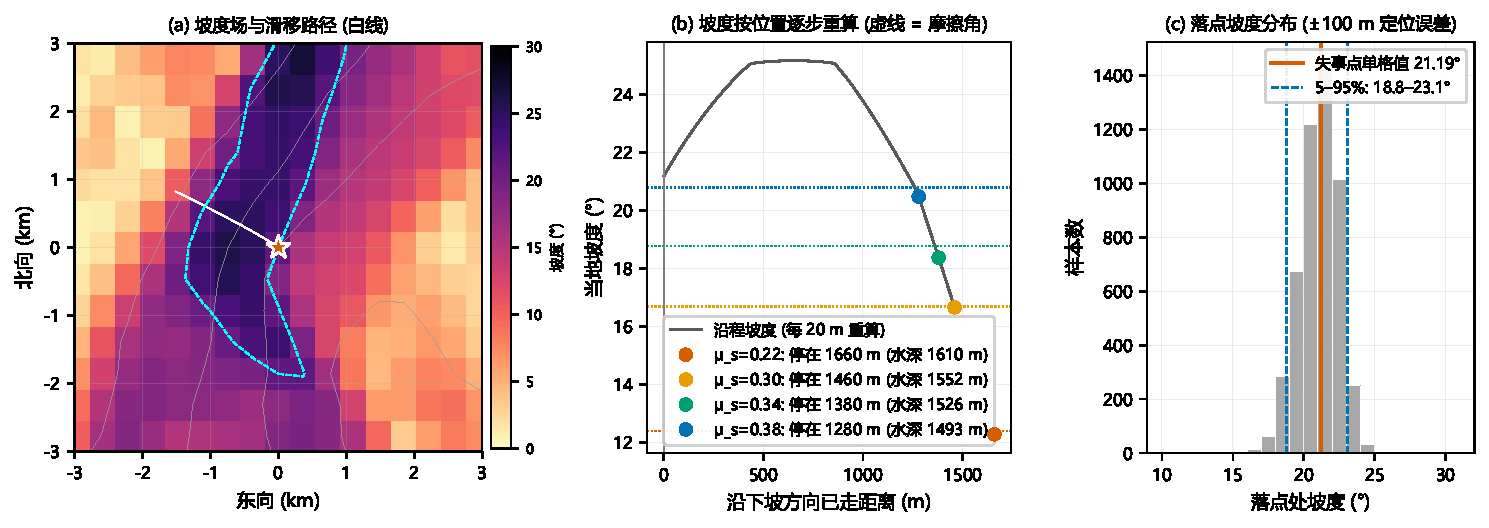
\includegraphics[width=0.84\textwidth]{fig_p2_slope}
\caption{海底滑移机制（主算例）。(a) 海域坡度与几条滑移路径；(b) 单条滑移路径上
每 20 m 重算的坡度剖面与 $\mu_s$ 停止点；(c) 不同坡度下发生滑移的比例。}
\label{fig:slope}
\end{figure}

\subsection{数值算法}

\begin{enumerate}[leftmargin=1.8em,itemsep=0pt]
\item \textbf{惯性段}（$0\le t\le2$ h）：垂向用解析解~\eqref{eq:analytic}，步长 $\Delta t=10$ s
      （720 步），触底者立即执行滑移；
\item \textbf{漂流段}（$2<t\le96$ h）：垂向状态已稳定，步长 $\Delta t=900$ s（376 步），
      流场按四维插值；
\item 记录 97 个逐小时快照供搜索模型使用；同时记录水面/海底到达时刻与滑移距离。
\end{enumerate}

\subsection{压溃的事后统计}\label{sec:crush}

题目不允许把“压溃”当作确定的终止条件，因此模拟中\emph{不做压溃截断}：超过额定潜深的
粒子继续下沉，最后统一给出“给定假设压溃深度 $D_c$ 下，任意时刻超深概率”
$P(z(t)>D_c)$ 曲线。取 $D_c=1.5\times$ 额定潜深 = 1500 m（工程经验的安全裕度），
主算例中沉底分支终点水深中位数 1451 m，$P(\text{深度}>1000\text{ m})=9.7\%$、
$P(>1500\text{ m})=6.9\%$。这一处理既保留了题目要求的“不模拟压溃”，又能为后文
“A95 面积”与“搜救难度”提供一致的概率解释。

\subsection{验证}

模型共通过 5 项可复现的验证（\tabref{tab:verify}），全部可在代码中重跑。

\begin{table}[H]
\centering\small
\caption{定位模型的验证记录}
\label{tab:verify}
\begin{tabular}{@{}llll@{}}
\toprule
项目 & 方法 & 判据 & 结果\\
\midrule
海水状态方程 & EOS-80 + Chen--Millero 与公开值对比 & 相对误差 $<10^{-4}$ & 通过\\
终端速度 & 解析解 vs 数值积分 & 相对误差 & 0.00\%\\
OU 过程 & 长时间方差 vs 理论值 $\sigma^2$ & 相对误差 $<5\%$ & 1.61\%\\
滑移判据 & 单一坡度解析 vs 逐 20 m 重算 & 停止位置一致 & 通过\\
地形插值 & 双线性 vs 最近邻（水深场） & 深度差 $<1$ m & 通过\\
\bottomrule
\end{tabular}
\end{table}

其中“滑移判据”验证的做法是：取 $\mu_s=0.35$（摩擦角 19.3°），在 20° 与 25° 两个
均匀坡度上分别用解析式与逐步法计算滑移距离，两者分别为 1340 m 与 1514 m，误差来自
逐步法在坡度变化处的重新判断，属预期行为。EOS-80 的验证覆盖 0--1000 m 压力范围，
与模型使用的深度范围一致。
